\documentclass[12pt]{article}
\usepackage[a4paper, total={7.5in, 11in}]{geometry}
\usepackage{array}
\usepackage{graphicx, subfig, wrapfig, fancyhdr, lastpage, multicol ,color,arydshln,makecell, chemfig}

\newcommand\headerMe[2]{\noindent{}#1\hfill#2}
\usepackage[mathscr]{euscript}
\usepackage{tabularray}

\setlength{\columnseprule}{1pt}
\def\columnseprulecolor{\color{blue}}


\pagestyle{fancy}
\fancyhf{}

\cfoot{ \vspace{-0.8cm}\em{Page \thepage \hspace{1pt} / \pageref{LastPage}}}
\begin{document}

\headerMe{Royaume du Maroc}{année scolaire \emph{2022-2023}}\\
\headerMe{Ministère de l'Éducation nationale, }{  Professeur :\emph{Zakaria Haouzan}}\\
\headerMe{du Préscolaire et des Sports}{Établissement : \emph{Lycée SKHOR qualifiant}}\\
%\vspace{-1cm}
\begin{center}
Devoir Surveillé  N°3 - S2 \\
    2ème année baccalauréat Sciences physiques\\
Durée 2h00
\\
    \vspace{.2cm}
\hrulefill
\Large{Chimie 7pts - 45min}
\hrulefill\\

    %\emph{Les deux parties sont indépendantes}
\end{center}
%end Headerss------------------------
%__________________Chimie ______________________-
%%%%%%%+_+_+_+_+_+_+_+_+_Partie1

 \section*{Partie 1 : Hydrolyse d’un Ester \dotfill(7pts)-45min }
%\begin{wrapfigure}{r}{0.16\textwidth}
	%\vspace{-1.2cm}
%%\begin{center}
  %%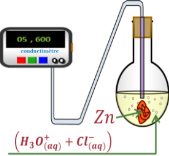
\includegraphics[width=0.16\textwidth]{./img/chimie01.png}
%%\end{center}
%\end{wrapfigure}
L’éthanoate de benzyle $CH_3-CO_2-CH_2-C_6H_5$ est un ester très parfumé extrait du jasmin. On recueille un échantillon presque pur.

\underline{Données:}
\begin{itemize}
	\item formule semi-développée de l’alcool benzylique : 
$\chemfig{*6(-=-(-CH_2-OH)=-()=)}$
\item masse molaire de l’éthanoate de benzyle : $150 g.mol^{-1}$
\end{itemize}
L’échantillon précédent est introduit dans un ballon avec une quantité de matière égale d’eau et quelques
gouttes d’acide sulfurique concentré. Ce ballon, équipé d’un chauffage à reflux, est placé au bain marie. La
\textbf{constante d’équilibre K de la réaction d’hydrolyse qui se produit est égale à 0,25}.

\hspace{-1cm} \textbf{1. Étude de la réaction d’hydrolyse.\dotfill}


\begin{tabular}{c | c}
		1 & \makecell[l]{\textbf{1.1. } Écrire, en utilisant les formules semi-développées, l’équation de la réaction. Nommer les\\ produits formés.}\\

		0,5 & \makecell[l]{\textbf{1.2. } Donner deux caractéristiques de cette réaction.\\ }

	
		\end{tabular}
			
						\hspace{-1cm}\textbf{2. Étude du montage.\dotfill}

\begin{tabular}{c|l}
	1  & \makecell[l]{ \textbf{2.1. } Schématiser le montage utilisé. Quel est l’intérêt de ce montage ?}\\

	0,5	 & \makecell[l]{\textbf{2.2. } Quel est le rôle de l’acide sulfurique ?}\\

\end{tabular}

						\hspace{-1cm}\textbf{3.On note $n_0$ les quantités de matière initiales des réactifs et $x_f$ l’avancement de la réaction dans l’état final..\dotfill}

\begin{tabular}{c|l}
	1  & \makecell[l]{ \textbf{3.1. } Dresser le tableau d’avancement de la réaction.}\\

	0,5	 & \makecell[l]{\textbf{3.2. } Définir le taux d’avancement $\tau$ de la réaction.}\\
	
	1	 & \makecell[l]{\textbf{3.3. } Donner l’expression de la constante d’équilibre K. Montrer que $K = \frac{\tau^2}{(1-\tau^2)}$}\\
	
	0,5	 & \makecell[l]{\textbf{3.4. } Vérifier que le rendement de la réaction est pratiquement égal à 33\%.}\\
	
	0,5	 & \makecell[l]{\textbf{3.5. } Déterminer la masse del’ester extrait pour $n_0 = 0,1mol$.}\\
	
	0,5	 & \makecell[l]{\textbf{4. } Comment évolue le rendement de la réaction lorsqu’on extrait l’alcool du milieu réactionnel.}\\

\end{tabular}
%\hrulefill
%\Large{Physique 13pts/78min}
%\hrulefill\\
%\newpage
\begin{center}
    %\vspace{.60cm}
\hrulefill
\Large{Physique 13pts - 75min}
\hrulefill\\
    \emph{Les  parties sont indépendantes}
\end{center}

%\vspace{-1cm}
\section*{Partie 1 : Pendule de Torsion \dotfill(6,00pts)}






Un Pendule de torsion est constitué d'un fil d'acier de constante de torsion C et une barre homogène AB de Longueur L, suspendue à ce fil en son centre O (figure 1).

\begin{wrapfigure}[1]{r}{0.3\textwidth}
\begin{center}
  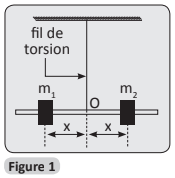
\includegraphics[width=0.2\textwidth]{./img/ex02.png}
  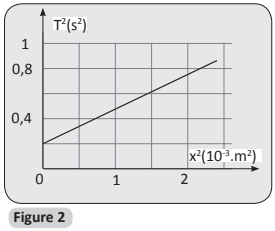
\includegraphics[width=0.3\textwidth]{./img/ex021.png}
\end{center}
\end{wrapfigure}

Son moment d'inertie par rapport à l'axe $(\Delta)$ confondu avec le fil est $J_0$.
\begin{itemize}
	\item A la même distance x de l'axe, on fixe sur la tige deux masselottes $(S_1)$ \\et $(S_2)$ \\de masses $m_1$=$m_2$=$m$=$100g$.
	\item Le moment d'inertie du système ainsi constitué {AB + ($S_1$)($S_2$)}. a pour \\expression $J_{\Delta} = J_0 +2.m.x^2$.
	\item On écarte la barre de sa position d'équilibre, dans le plan \\horizontal ,jusqu'à l'angle  $\theta = \frac{\pi}{6}rad$ et on l'abandonne sans vitesse\\ à une date $t_0 = 0s$

	\item On néglige  les frottement et on prend $\pi^2 = 10$.
\end{itemize}

\begin{tabular}{c|l}

	1,5 & \makecell[l]{\textbf{1. } à l'aide d'une étude dynamique, établir que $\ddot{\theta} + \frac{C}{J_{\Delta}}.\theta$}\\

	1 & \makecell[l]{\textbf{2. } Ecrire l’équation horaire du mouvement du pendule.}\\
	
	1,5 & \makecell[l]{\textbf{3. } Montrer que : $T_0^2 = \frac{4.\pi^2.J_0}{C} + \frac{8.\pi^2.m}{C}.x^2$}\\
	
\end{tabular}



\hspace{-1cm} \textbf{4. } On fait varier la distance $x$ et on mesure à l'aide d'un \\chronométre la période $T_0$. Les résultats obtenus ont abouti à la courbe  de la figure (2) En exploitant cette figure.
	
\begin{tabular}{c|l}
	1 & \makecell[l]{\textbf{4.1 } Déterminer la valeur de la constante de torsion C.}\\
	1 & \makecell[l]{\textbf{4.2 } Déterminer la valeur du moment d'inertie $J_0$ de la barre $AB$.}\\
	\end{tabular}

	\section*{Partie 2 : Oscillateur mécanique simple. \dotfill(4pts)}

%\begin{wrapfigure}[9]{r}{0.25\textwidth}
  %\begin{center}
	  %\vspace{-1cm}
	%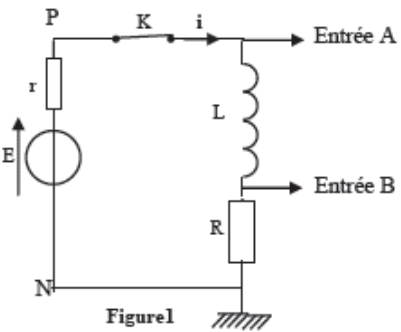
\includegraphics[width=0.22\textwidth]{./img/img03.png}
	%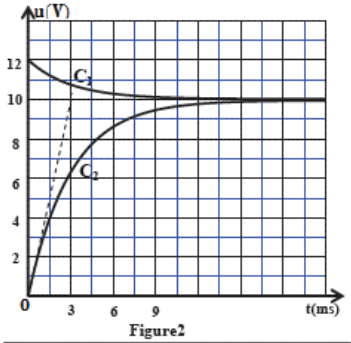
\includegraphics[width=0.25\textwidth]{./img/img04.png}
  %\end{center}
%\end{wrapfigure}

\begin{wrapfigure}[6]{r}{0.15\textwidth}
\begin{center}
	\vspace{-1.6cm}
  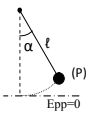
\includegraphics[width=0.15\textwidth]{./img/ex03.png}
\end{center}
\end{wrapfigure}


\emph{Le but de cette étude est de trouver la condition à
satisfaire pour qu'un pendule simple puisse être considéré
comme un oscillateur harmonique.
Rappel : L’équation différentielle vérifiée par un
oscillateur harmonique est de la forme : $\ddot{y} + \omega_0^2.y = 0$}

Un pendule simple (P) est formé d'une petite boule, de
masse $m = 200 g$, suspendue à un fil de masse négligeable
et de longueur $l = 1 m$. (P) est écarté
d'un angle $\alpha_m$ par rapport à la
position d'équilibre, est lâché sans
vitesse initiale à la date $t_0 = 0$. À un
instant t, (P) est repéré par l’angle $\alpha$
et se déplace à la vitesse V.
On prend $g = 10 m/s^2$ et on néglige
toutes les forces de frottement.


\hspace{-1cm} \textbf{1. Étude théorique.\dotfill}
	\begin{tabular}{c|l}	

	1,5 & \makecell[l]{\textbf{1. } La position la plus basse de la boule est prise comme
niveau zéro de l'énergie potentielle de \\pesanteur. À la
date t, établir l'expression suivante de l'énergie
mécanique $E_m$ du système \\((P), Terre) : $E_m=\frac{1}{2}.m.l^2.\dot{\alpha^2} + mgl(1- cos\alpha)$}\\

		1,75 & \makecell[l]{\textbf{2. } En appliquant la conservation de $Em$, montrer que: $\dot{\alpha}^2 = \frac{2.g}{l}.(cos\alpha - cos\alpha_m)$ }\\

	0,75 & \makecell[l]{\textbf{3. } Déduire alors l'expression de la période propre $T_0$ de
ce pendule harmonique et calculer sa valeur.\\ $(sin(\alpha) \approx \alpha$)}
\end{tabular}


	\section*{Partie 3 : Atome d'hydrogène \dotfill(2,50pts)}

\begin{wrapfigure}[6]{r}{0.24\textwidth}
\begin{center}
	\vspace{-0.6cm}
  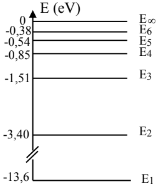
\includegraphics[width=0.24\textwidth]{./img/ex04.png}
\end{center}
\end{wrapfigure}

La figure ci-contre montre le
diagramme énergétique de
quelques niveaux d'énergie En
d'un atome d'hydrogène.

\textbf{Données:} $c = 2,998.10^8 m/s$ ; $h = 6,626.10^{-34} J.s; 1 eV = 1,60.10^{-19}J$

	\begin{tabular}{c|l}	

	0,5 & \makecell[l]{\textbf{1. } Dans quel état se trouve l'atome lorsque son énergie
est null?}\\

		0,5 & \makecell[l]{\textbf{2. } Dans ce cas, l'électron de cet atome est-il lié ou libre?}\\

	0,75 & \makecell[l]{\textbf{3. } Déterminer l'énergie d'ionisation de l'atome
	d'hydrogène pris \\dans l'état fondamental.}\\	
		0,75 & \makecell[l]{\textbf{4. } Montrer que l'absorption d'une radiation de longueur
d'onde \\$\lambda = 91,20 nm$ fait passer l'atome du niveau
fondamental \\à l'état ionisé.}
\end{tabular}




	%\vspace{0.5cm}
%\textbf{2. Injection locale d’une solution contenant du rhénium 186.
%Le produit injectable se présente sous la forme d’une solution contenue dans un flacon de volume $V_0= 10 mL$ ayant une activité $a_0 = 4.10^9Bq$ à la date $t=0$, c'est-à-dire à la sortie du laboratoire pharmaceutique.}
	%\begin{tabular}{c|l}

		%1 & \makecell[l]{\textbf{2.1 }Déterminer en jours la valeur de demi-vie $t_{1/2}$ du rhénium $_{75}^{186}Re$}\\

		%0,5 & \makecell[l]{\textbf{2.2 }Trouver, à l’instant $t_1 = 4,8jours$, le nombre $N_1$ de noyau de rhénium contenu dans le flacon.}\\

		%0,5 & \makecell[l]{\textbf{3.2 } À l’instant $t_1$ on prélève du flacon de volume $V_0 = 10mL$ une injection de volume V contenant \\$N = 3,65.10^{13}$ noyaux de rhénium 186, on l’injecte à un malade dans l’articulation de l’épaule, \\trouver la valeur de V.}\\
	%\end{tabular}


%\section*{Partie 2 :  Centrale nucléaire \dotfill(9pts)}
%Dans une centrale nucléaire, les noyaux d'uranium $^{235}_{92}U$ subissent la fission sous le choc d'un neutron
%lent. Un des nombreux processus possibles conduit à la formation d'un noyau de lanthane $^{144}_{57}La$ ,d'un noyau de brome $^{88}_{35}Br$ et  de plusieurs neutrons.

%\begin{tabular}{c|l}

 %1& \makecell[l]{\textbf{1. } Définissez l'énergie de liaison d'un noyau.}\\

 %1 & \makecell[l]{\textbf{2. } Donnez l'expression littérale qui permettra son calcul.}\\

 %1 & \makecell[l]{\textbf{3. } Calculez, en MeV, l'énergie de liaison d’un noyau $^{235}_{92}U$.}\\

 %1 & \makecell[l]{\textbf{4. } Calculez l’énergie de liaison par nucléon de ce noyau.}\\

 %1 & \makecell[l]{\textbf{5. } Ecrivez l’équation de la réaction de fission étudiée.}\\

 %1 & \makecell[l]{\textbf{6. } Exprimez l'énergie libérée par la fission d'un noyau $^{235}_{92}U$ en fonction des énergies de liaison par
%\\ nucléon du noyau père et des noyaux fils et calculez la valeur de cette énergie en MeV.}

 %\end{tabular}

%\textbf{7.  Dans le cœur de la centrale, de nombreuses autres réactions de fission du noyau $^{235}_{92}U$ se produisent. La perte de masse est, en moyenne, de 0,200 u par noyau.}


%\begin{tabular}{c|l}

	%1,5 & \makecell[l]{\textbf{7.1. } Calculez, en MeV, l'énergie moyenne libérée par la fission d’un noyau. Ce résultat est-il \\en concordance avec celui de la question 6 ?}\\

	%1,5 &\makecell[l]{\textbf{7.2. }Calculez, en joule, l'énergie moyenne libérée par une mole de noyaux $^{235}_{92}U$ } 

%\end{tabular}

%\textbf{Données :}
%\begin{itemize}
	%\item Célérité de la lumière dans le vide : $c = 2,998 . 10^8 m.s^{-1}$  
	%\item Masse du noyau d’uranium 235 : $m( ^{235}_{92}U) = 235,0134u$ 

	%\item Energies de liaison par nucléon : $E_l/A(^{144}_{57}La) = 8,28MeV/nucl$éon  ; $E_l/A(^{88}_{35}Br)$=$8,56MeV/nucl$éon
	%\item Constante d'Avogadro : $N_A = 6,02.10^{23} mol^{-1}$
	%\item $1u$ = $1,66055.10^{-27}Kg$ et $1eV = 1,602.10^{-19}J$
	%\item Masse d’un proton : $m(^1_1p) = 1,0073u$ ; Masse d’un neutron $m(^1_0n) = 1,0087u$
%\end{itemize}





\end{document}
